\documentclass{article}

% Language setting
% Replace `english' with e.g. `spanish' to change the document language
\usepackage[english]{babel}

% Set page size and margins
% Replace `letterpaper' with `a4paper' for UK/EU standard size
\usepackage[letterpaper,top=2cm,bottom=2cm,left=3cm,right=3cm,marginparwidth=1.75cm]{geometry}

% Useful packages
\usepackage{amsmath}
\usepackage{graphicx}
\usepackage[colorlinks=true, allcolors=blue]{hyperref}

% increase paragraph spacing
\usepackage[skip=10pt plus1pt]{parskip}
% increase line spacing
\renewcommand{\baselinestretch}{1.1} 

% to fix figure positions
\usepackage{float}

% to create nice-looking tables
\usepackage{tabularx} 
\usepackage{graphicx} 
\usepackage{subcaption} 
\usepackage{csvsimple} %%%%%%%%%%%%%%%%%%%%%%%%%%%%%%%%%%%%
\usepackage{booktabs}%%%%%%%%%%%%%%%%%%%%%%%%%%%%%%%%%%%%
\usepackage{adjustbox} % Add this package

% to use Matlab code in text (by Min)
\usepackage{fancyhdr}
\pagestyle{fancy}
\usepackage{listings}

% To write code formatting
\newcommand{\code}[1]{\texttt{#1}}

\title{Dimension reduction techniques in linear regression}
\author{Ismael Ahmad Rab}

\begin{document}
\maketitle


\section*{Abstract}

Dimension reduction techniques are used in order to visualise and extract meaningful insights from high dimensional data by projecting it into lower dimensional systems. Principal Component Analysis (PCA) is one of the most known tools. It is based on finding an orthonormal basis of the data which captures most of the information's variance with the least amount of 'directions'. The new coordinate system is easily expressed in terms of the original variables, offering interpretability. However, in the context of supervised learning, PCA is greatly limited by the fact that it doesn't involve the target variable. There are various techniques based on PCA which try to perform interpretable feature engineering while maximising predictive power. In this project we explore such techniques in the context of linear regression and explore how regularisation methods can be used for this task.

\section{Introduction}

Principal Component Regression (PCR) \cite{Massy1965}, is a two-stage procedure by which PCA is applied to the features, and the first m Principal Components (PCs) are used as the predictors in a linear regression model. Although PCs capture the variability of the features it does not necessarily do the same for the response variable. A solution to this would be making use of the target when computing the PCs. One-stage procedures such as Partial Least Squares Regression (PLSR) \cite{Wold1966} and Sparse Principal Component Regression (SPCR) \cite{SPCR2018} are able to incorporate the response into the computation of the projections. We consider a (n,p) feature matrix X and response variable Y.

\section{Techniques}

\subsection{Principal Component Regression}
PCR aims to predict the response variable by considering the first l PCs which capture most of the variability, $\{\Gamma_{i}\;|\;i = 1,...,l\}$ as the features used in linear regression, where $l$ is usually chosen through cross-validation. This method relies in the PCs being the best directions for explaining the response, which is not a necessarily true. If Y is highly correlated with PCs corresponding to smaller eigenvalues, we would either loose explainability wrt to the response or need to consider a high number of PCs which would defeat the purpose of the technique. Furthermore, the problem with this technique is that redundant variables wrt the target might be included in the PCs which capture the most variance, leading to possibly erratic estimates wrt the original variables.

\subsection{Partial Least Squares Regression}
Two-stage techniques which begin with PCA, such as PCR, suffer from the fact that PCs are computed without considering the response variable. Wold proposed a single-stage method, PLSR \cite{Wold1966}, where orthogonal linear combinations of the original predictors which best explain the variance in the predictors and the response are computed iteratively, and at each step the contribution of the corresponding 'direction' is removed from the feature and response arrays. Similarly to PCR, once the new projections are found, linear regression is performed using the first $l$ PCs which capture the most variability as the features, with $l$ usually being found via cross-validation.

\subsection{Sparse Principal Component Regression}
In \cite{SPCR2018} another single-stage method was proposed. It is based on the idea of Sparse Principal Component Analysis (SPCA) \cite{SPCA}. In the former article PCA is formulated as the following regression problem: 

\vspace{-2.5em}

\begin{center}
    $$\displaystyle\min_{B}\sum_{i=1}^{n}||\boldsymbol{x_{i}}-BB^{T}\boldsymbol{x_{i}}||\;\;\;\text{subject to: $BB^{T} = I$}$$
\end{center}

\vspace{-1em}

Where $\boldsymbol{x_{i}}$ corresponds to the i-th row of the feature matrix, X, and B corresponds to the loading matrix. Conditions are relaxed and terms corresponding to elastic net regularisation are introduced to penalise the size of the corresponding loadings at the cost of orthonormality. The reasoning is that due to the nature of PCA it is rather difficult for predictors to contribute exactly 0 towards a principal component, but through regularisation we may achieve this.

SPCR extends this by considering the formulation mentioned above together with least squares linear regression, combining them in order to consider sparse loadings and the response variable. In particular, the objective function to minimise in SPCR is:

\vspace{-2.5em}

\begin{center}
    $$\displaystyle\min_{A,B, \gamma_{0}, \boldsymbol{\gamma}}\;\;\;\sum_{i=1}^{n}(y_{i}-\gamma_{0}-\boldsymbol{\gamma^{T}}B^{T}\boldsymbol{x_{i}})^{2} + w\sum_{i=1}^{n}||\boldsymbol{x_{i}} - AB^{T}\boldsymbol{x_{i}}||_{2}^{2}$$\\
    $$+ \lambda_{\beta}\xi\sum_{j=1}^{p}||\boldsymbol{\beta}_{j}||_{2}^{2} + \lambda_{\beta}(1-\xi)\sum_{j=1}^{p}||\boldsymbol{\beta}_{j}||_{1} + \lambda_{\gamma}||\boldsymbol{\gamma}||_{1}\;\;\;\text{subject to: $A^{T}A = I$}$$
\end{center}

Where $\gamma_{0}, \boldsymbol{\gamma}$ correspond to the estimated coefficients from regressing the response using the projection of the features, and $\lambda_{\beta}, \lambda_{\gamma}, w$ and $\xi$ are regularisation or tuning parameters. 

The first term corresponds to the squared loss function of the linear regression using the projected features, the second term is the loss function presented and used in \cite{SPCA} for SPCA, where the absence of B and presence of matrix A corresponds to relaxing conditions at the loss of orthogonality of the loading vectors ($\boldsymbol{\beta}_{j}$ corresponds to the i-th column of B). The third and fourth terms represent the elastic net computation of the loadings used in the projections, which is done for the sake of sparsity. It should be noted that elastic net is used due to possible correlations between the original variables (highly correlated variables can share a coefficient value infinitely many ways, and the L1 norm does not distinguish between them, leading to erratic and sensible behaviour when "deciding" which variable to discard, while the L2 norm will make such variables share the coefficient value equally \cite{SL_sparsity}). The last term corresponds to a L1 penalty added to the estimated coefficients. 

Sparsity in the loading vectors will result in more interpretable projections of the data and due to he least squares error it should be induced over the superfluous variables wrt the response. Moreover, the L1 penalty over the regression coefficients ($\boldsymbol{\gamma}$) may introduce automatic variable selection in the new projections. There are various drawbacks to this method, including a great computational cost for large sample sizes. Moreover, the number of projections to consider is to be chosen by the user.

\section{Implementation and Simulation}
PCR and PLSR are both implemented in R through the \code{pls} package, the corresponding functions include cross-validation for selecting the optimal number of PCs to use. SPCR is implemented in the \code{spcr} package, however it only allows for cross-validation in order to find the regularisation parameters: $\lambda_{\beta}$ and $\lambda_{\gamma}$. In our implementation we alter the function so that cross-validation is used in order to find optimal values for $\lambda_{\beta}, \lambda_{\gamma}$ and the number of projections to consider.

We perform a simulation study by which we simulate 100 samples of the same population, each sample having 100 rows. For the population we consider 10 variables simulated using the multivariate normal distribution. All variables have mean 0 and the covariance matrix used to define the population is:

\begin{table}[htbp]
    \centering
    \caption{Matrix of Covariances}
    \resizebox{7cm}{!}{%
        \csvautotabular{static/covariance_matrix.csv}
    }
\end{table}

In particular, variables X1 to X4 are independent (minimal correlation between them). The rest of the variables are meant to introduce noise. In particular X5 is strongly correlated to X1, X6 is strongly correlated to X2, and X7 to X10 are minimally correlated with the first four variables, with X9 and X10 being strongly correlated amongst themselves. Furthermore, the response variable is generated through a linear relation defined by the following coefficient values:

\begin{table}[htbp]
    \centering
    \caption{True coefficient values}
    \resizebox{!}{0.45cm}{%
        \csvautotabular{static/coefficients.csv}
    }
\end{table}

Where noise/error is introduced through a random normal vector with mean 0, standard deviation 1.5 and which is of the same size as the number of rows per sample. The results of the simulations for the three methods presented are as follows:

\begin{figure}[H]
    \centering

    \begin{subfigure}{0.4\textwidth}
        \centering
        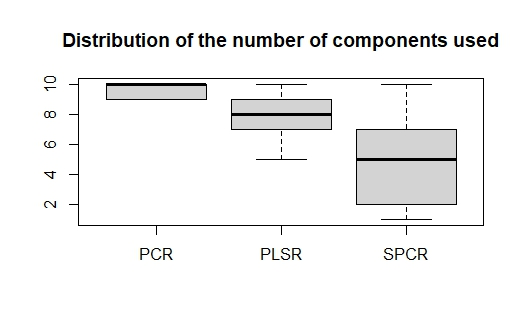
\includegraphics[width=85mm]{static/comps_dist.jpeg}
        \caption{Distribution of number of PCs used}
        \label{subfig:dist_ncomp}
    \end{subfigure}
    \hfill
    \begin{subfigure}{0.4\textwidth}
        \centering
        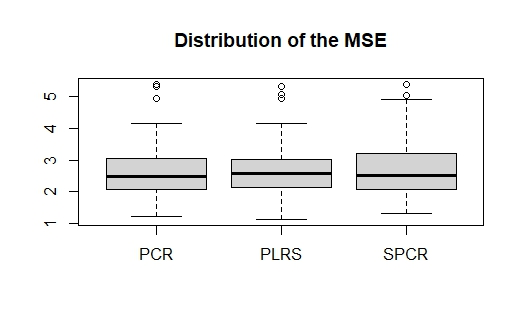
\includegraphics[width=85mm]{static/MSE_dist.jpeg}
        \caption{Distribution of MSE}
        \label{subfig:dist:MSE}
    \end{subfigure}

    \caption{Distribution of results per method}
    \label{fig:dist}
\end{figure}

From figure \ref{fig:dist} we can quickly see that PCR and PLSR are much more consistent in the number of components used, with PCR using (on average) the largest number of components. SPCR ranges across all possible values, using (on average) less projections. By looking at figure \ref{subfig:dist:MSE}, it is clear that PLSR is a great improvement from PCR, offering  almost identical predictive capabilities with (on average) less dimensions. SPCR reduces the number of projections, but at a loss of some predictive power. Furthermore, recall that SPCR looses the advantage of orthonormal projections, however due the sparsity gained from its SPCA term it generally leads to more interpretable projections when considered as linear combinations of the original variables due to the sharp 0s it will produce in the loading vectors.

\begin{figure}[H]
    \centering

    \begin{subfigure}{0.4\textwidth}
        \centering
        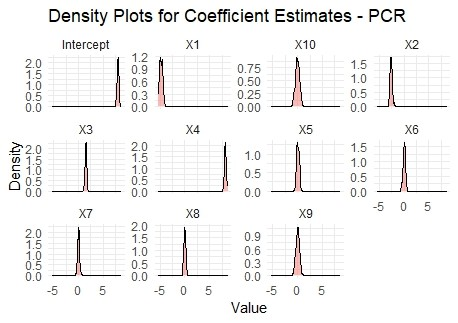
\includegraphics[width=85mm]{static/coff_dist_pcr.jpeg}
        \caption{Density Plot of PCR Coefficients}
        \label{subfig:dist_coeff_pcr}
    \end{subfigure}
    \hfill
    \begin{subfigure}{0.4\textwidth}
        \centering
        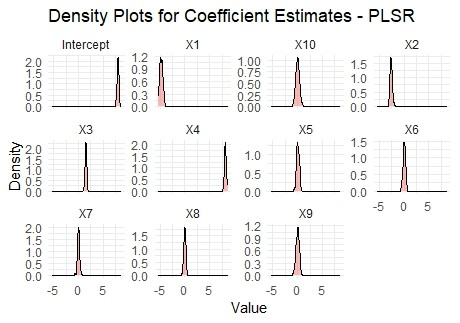
\includegraphics[width=85mm]{static/coff_dist_plsr.jpeg}
        \caption{Density Plot of PLSR Coefficients}
        \label{subfig:dist_coeff_plsr}
    \end{subfigure}

    \caption{Distribution of coefficients for PCR and PLSR}
    \label{fig:dist_coeffs}
\end{figure}

\begin{figure}[H]
    \centering
    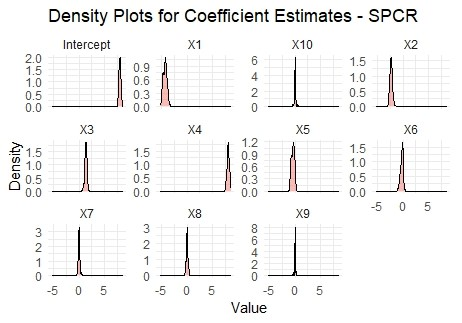
\includegraphics[height=65mm]{static/coff_dist_spcr.jpeg}
    \caption{Density Plot of PLSR Coefficients}
    \label{fig:dist_coeff_spcr}
\end{figure}

\begin{table}[htbp]
    \centering
    \caption{Distribution of coefficient values - PCR}
    \begin{adjustbox}{width=15cm, height=0.8cm}
        \begin{tabular}{c|c|c}
             \csvautotabular{static/coeff_info_pcr.csv}
        \end{tabular}
    \end{adjustbox}
\end{table}

\begin{table}[htbp]
    \centering
    \caption{Distribution of coefficient values - PLSR}
    \begin{adjustbox}{width=15cm, height=0.8cm}
        \begin{tabular}{c|c|c}
             \csvautotabular{static/coeff_info_plsr.csv}
        \end{tabular}
    \end{adjustbox}
\end{table}

\begin{table}[htbp]
    \centering
    \caption{Distribution of coefficient values - SPCR}
    \begin{adjustbox}{width=15cm, height=0.8cm}
        \begin{tabular}{c|c|c}
             \csvautotabular{static/coeff_info_spcr.csv}
        \end{tabular}
    \end{adjustbox}
\end{table}

From the distribution of coefficients (in terms of the original variables) we can see that SPCR does seem to lead to biased estimates, at least for the variables that are actually involved in generating the response, with an increased variance for these. Furthermore, it does not manage to deduce that, although heavily correlated with X1 and X2, X5 and X6 are not part of the response generation, while PCR and PLSR do seem to capture this. On the other hand it does a much better job in capturing the fact that variables X7 and X10 are essentially noise as the mean value for the estimates are similar to that of the other methods, but with smaller variance.



\bibliographystyle{apalike}
\bibliography{sample}

\end{document}